\clearpage
\subsection{Program} % (fold)
\label{sub:program}

A program contains the instructions the computer will follow when that program is executed. In your source code you can declare a program in which you code the steps you want followed when your program is executed. When you compile this code the compiler will create an executable file (a \emph{program}) that the user can run. Running the program will then get the computer to perform the steps you wrote in the code.

\begin{figure}[h]
   \centering
   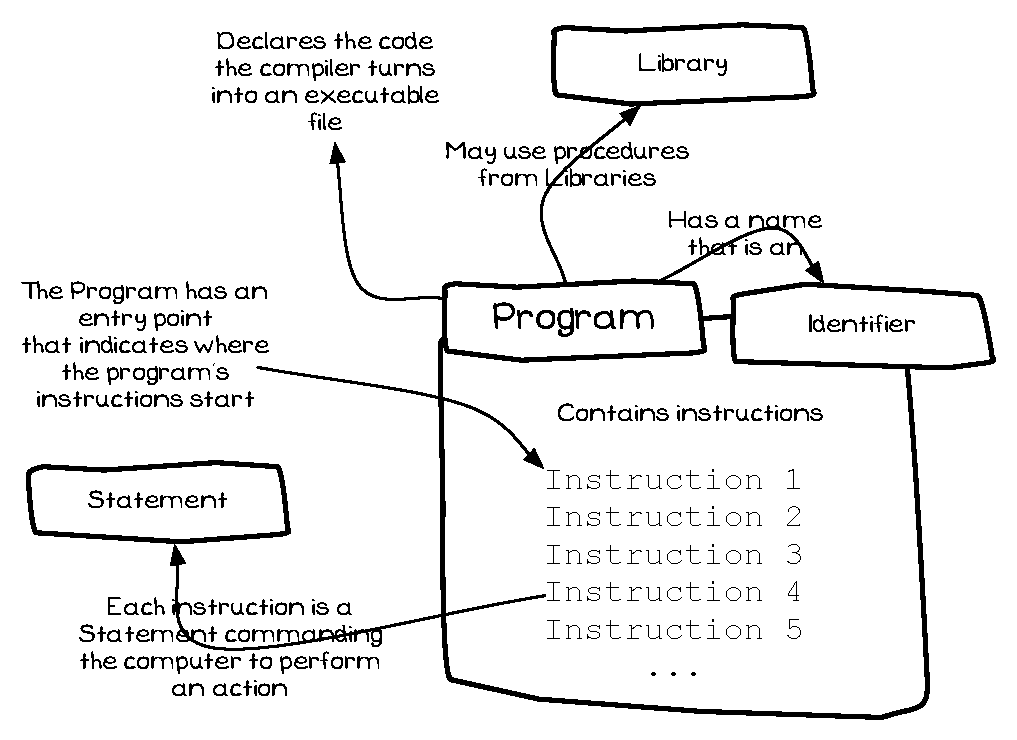
\includegraphics[width=\textwidth]{./topics/program-creation/diagrams/BasicProgramConcept} 
   \caption{A program contains instructions that command the computer to perform actions}
   \label{fig:program-creation-program}
\end{figure}


\mynote{
\begin{itemize}
  \item A program is an \textbf{artefact}, something you can create in your code.
  \item Figure \ref{fig:program-creation-program} shows the concepts related to programs.
  \item A program is a programming artefact used to define the steps to perform when the program is run.
  \item You use the compiler to convert the program's source code into an executable file.
  \item By declaring a program in your code you are telling the compiler to create a file the user can run.
  \item The program has an \textbf{entry point} that indicates where the program's instructions start.
  \item The name of the program determines the name of the executable file.
  \item Your program can use code from a \nameref{sub:library} or number of libraries.
  \item In programming terminology, an instruction is called a \nameref{sub:statement}.
\end{itemize}
}

% section program (end)